\chapter{Test Setup}
\label{chap:\currfilebase}

In the experiments conducted for this thesis, thin cuboid specimens were put under compressive force in direction of their long side. The force was induced in form of Combined Loading Compression (CLC), i.e. the compressive force was induced by both end- and shear-loading as shown in \autoref{fig:specimen_loads}.

\begin{figure}[!ht]
    \centering
    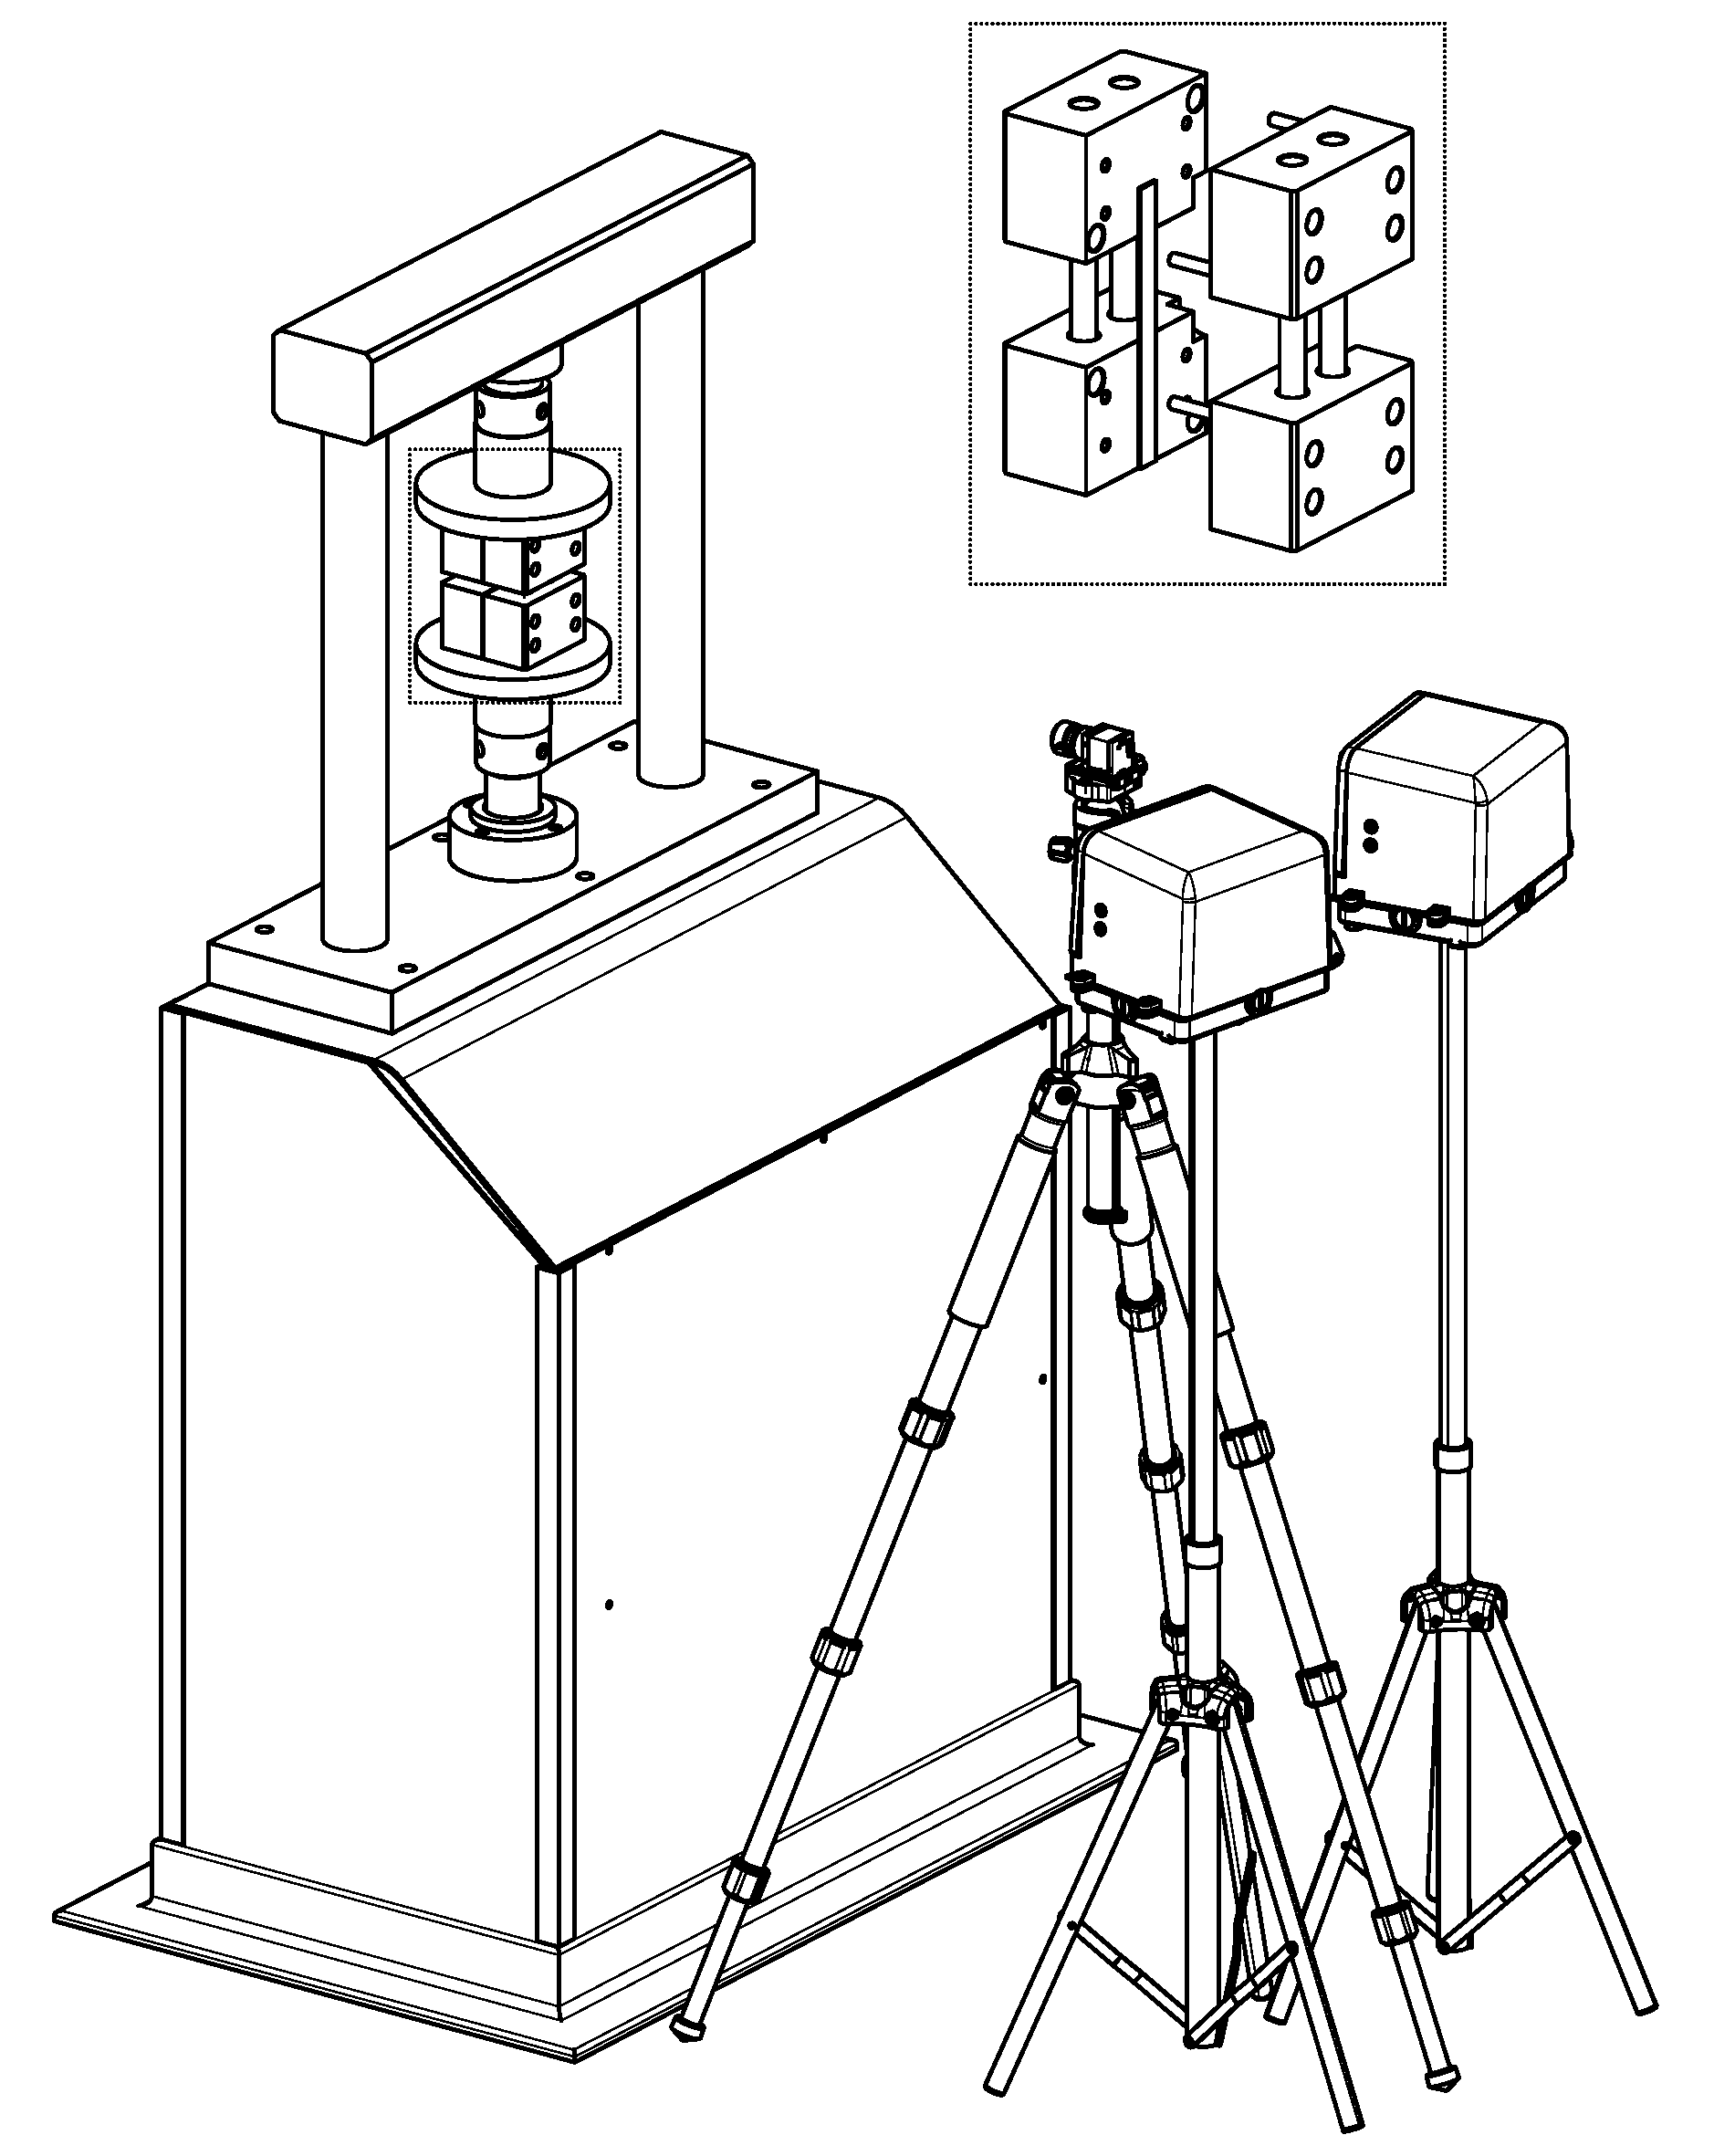
\includegraphics[scale=0.25]{\imgpath/\currfilebase/test_setup_scematic}
    \caption{Scematic of Test setup}
    \label{fig:test_setup_scematic}
\end{figure}

The test setup used consists of:
\begin{itemize}
    \item the test specimen
    \item a fatigue test system generating and measuring load and displacement
    \item a test fixture, transmitting the load of the test system to the specimen
    \item a CCD camera setup with the camera itself, a lens and light sources mounted on tripods
    \item a PC with software that allows synced recording of the fatigue test system and the CCD camera
\end{itemize}

Where the fatigue test system used was an instron 8801 in displacement-controlled mode and the CLC test fixture in use was an ASTM D6641 as depicted in \autoref{fig:sketch_clc_fixture}. The shear loading on the specimen is applied by increasing the torque of the clamping screws. The setup follows the recommendations of the test fixture standard \cite{D6641standard}.

\begin{figure}[!ht]
    \centering
    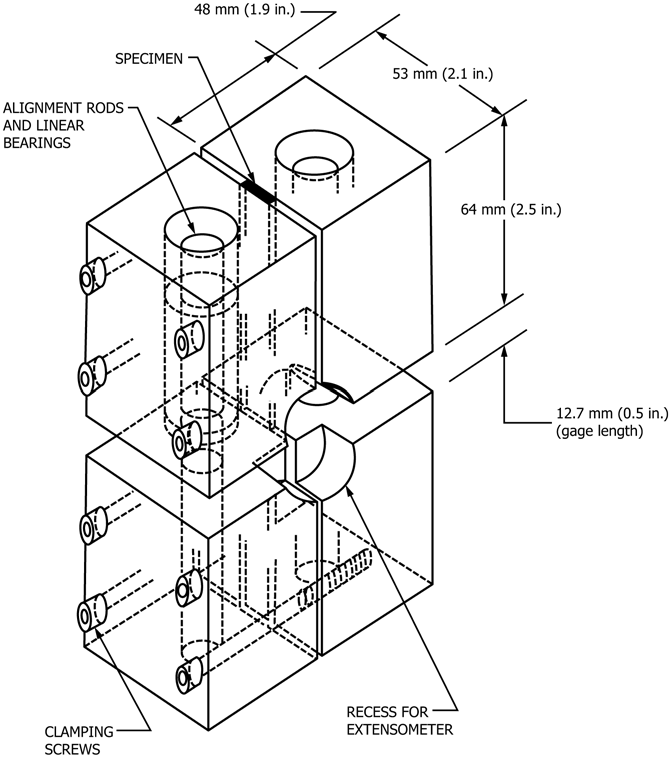
\includegraphics[scale=0.4]{\imgpath/\currfilebase/test_fixture.png}
    \caption{Dimensional Sketch of a Typical Combined Loading Compression (CLC) Test Fixture from \cite{D6641standard}}
    \label{fig:sketch_clc_fixture}
\end{figure}

\section{Specimen}
\label{sec:specimen}

The material used in the experiments is a unidirectional carbon fibre composite, i.e. a flat plate has been cured from thermoset prepregs\footnote{TC250 Resin System in unidirectional tape format} using vacuum bag and autoclave. The specimens were then shaped by water jet cutting this plate. An example cutting pattern is shown in \autoref{fig:specimen_plateA}, Where a bridge on each specimen circumference, connecting the base plate and the specimen, was not cut through to avoid the loss of specimens.
The Specimens were cut out in different angles with respect to the fibre direction. These angles are equal to the respective off-axis angles to the compressive loading direction in the setup if one neglects positioning inaccuracies.

For later identification, the specimens were labeled according to the test off-axis angle $\theta$, a plate identifier and a unique index.

\begin{figure}[!ht]
    \centering
    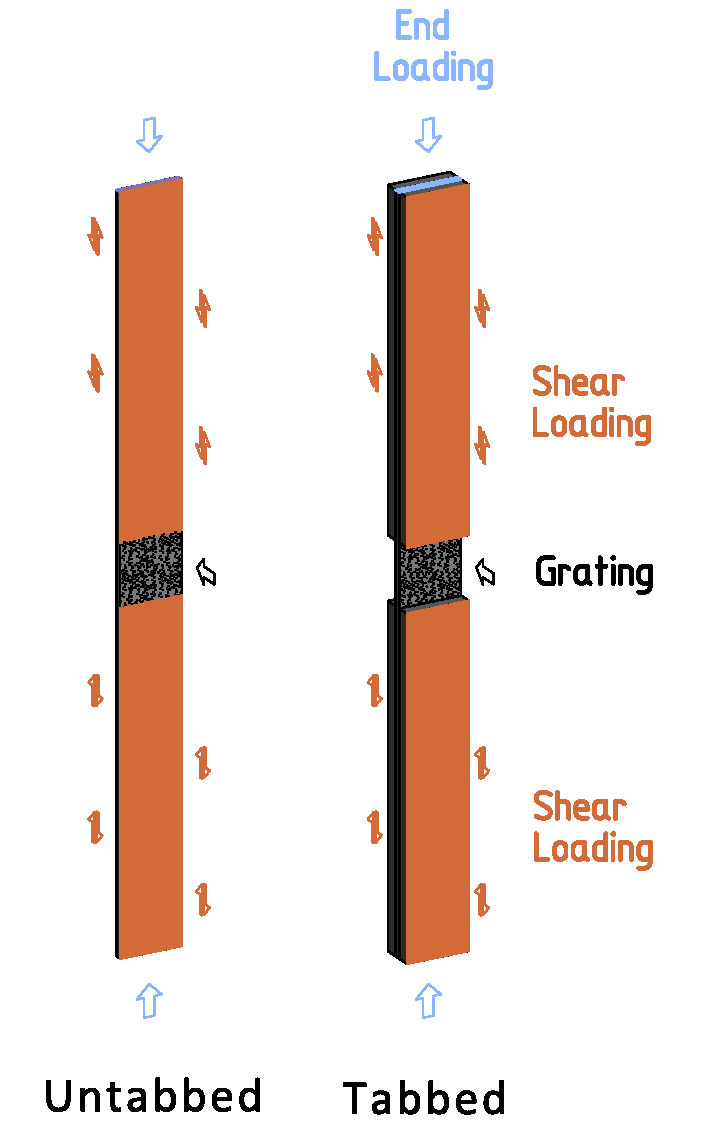
\includegraphics[scale=0.5]{\imgpath/\currfilebase/specimen_loads}
    \caption{Loads acting on both untabbed and tabbed specimens in setup respectively}
    \label{fig:specimen_loads}
\end{figure}
\begin{figure}[!ht]
    \centering
    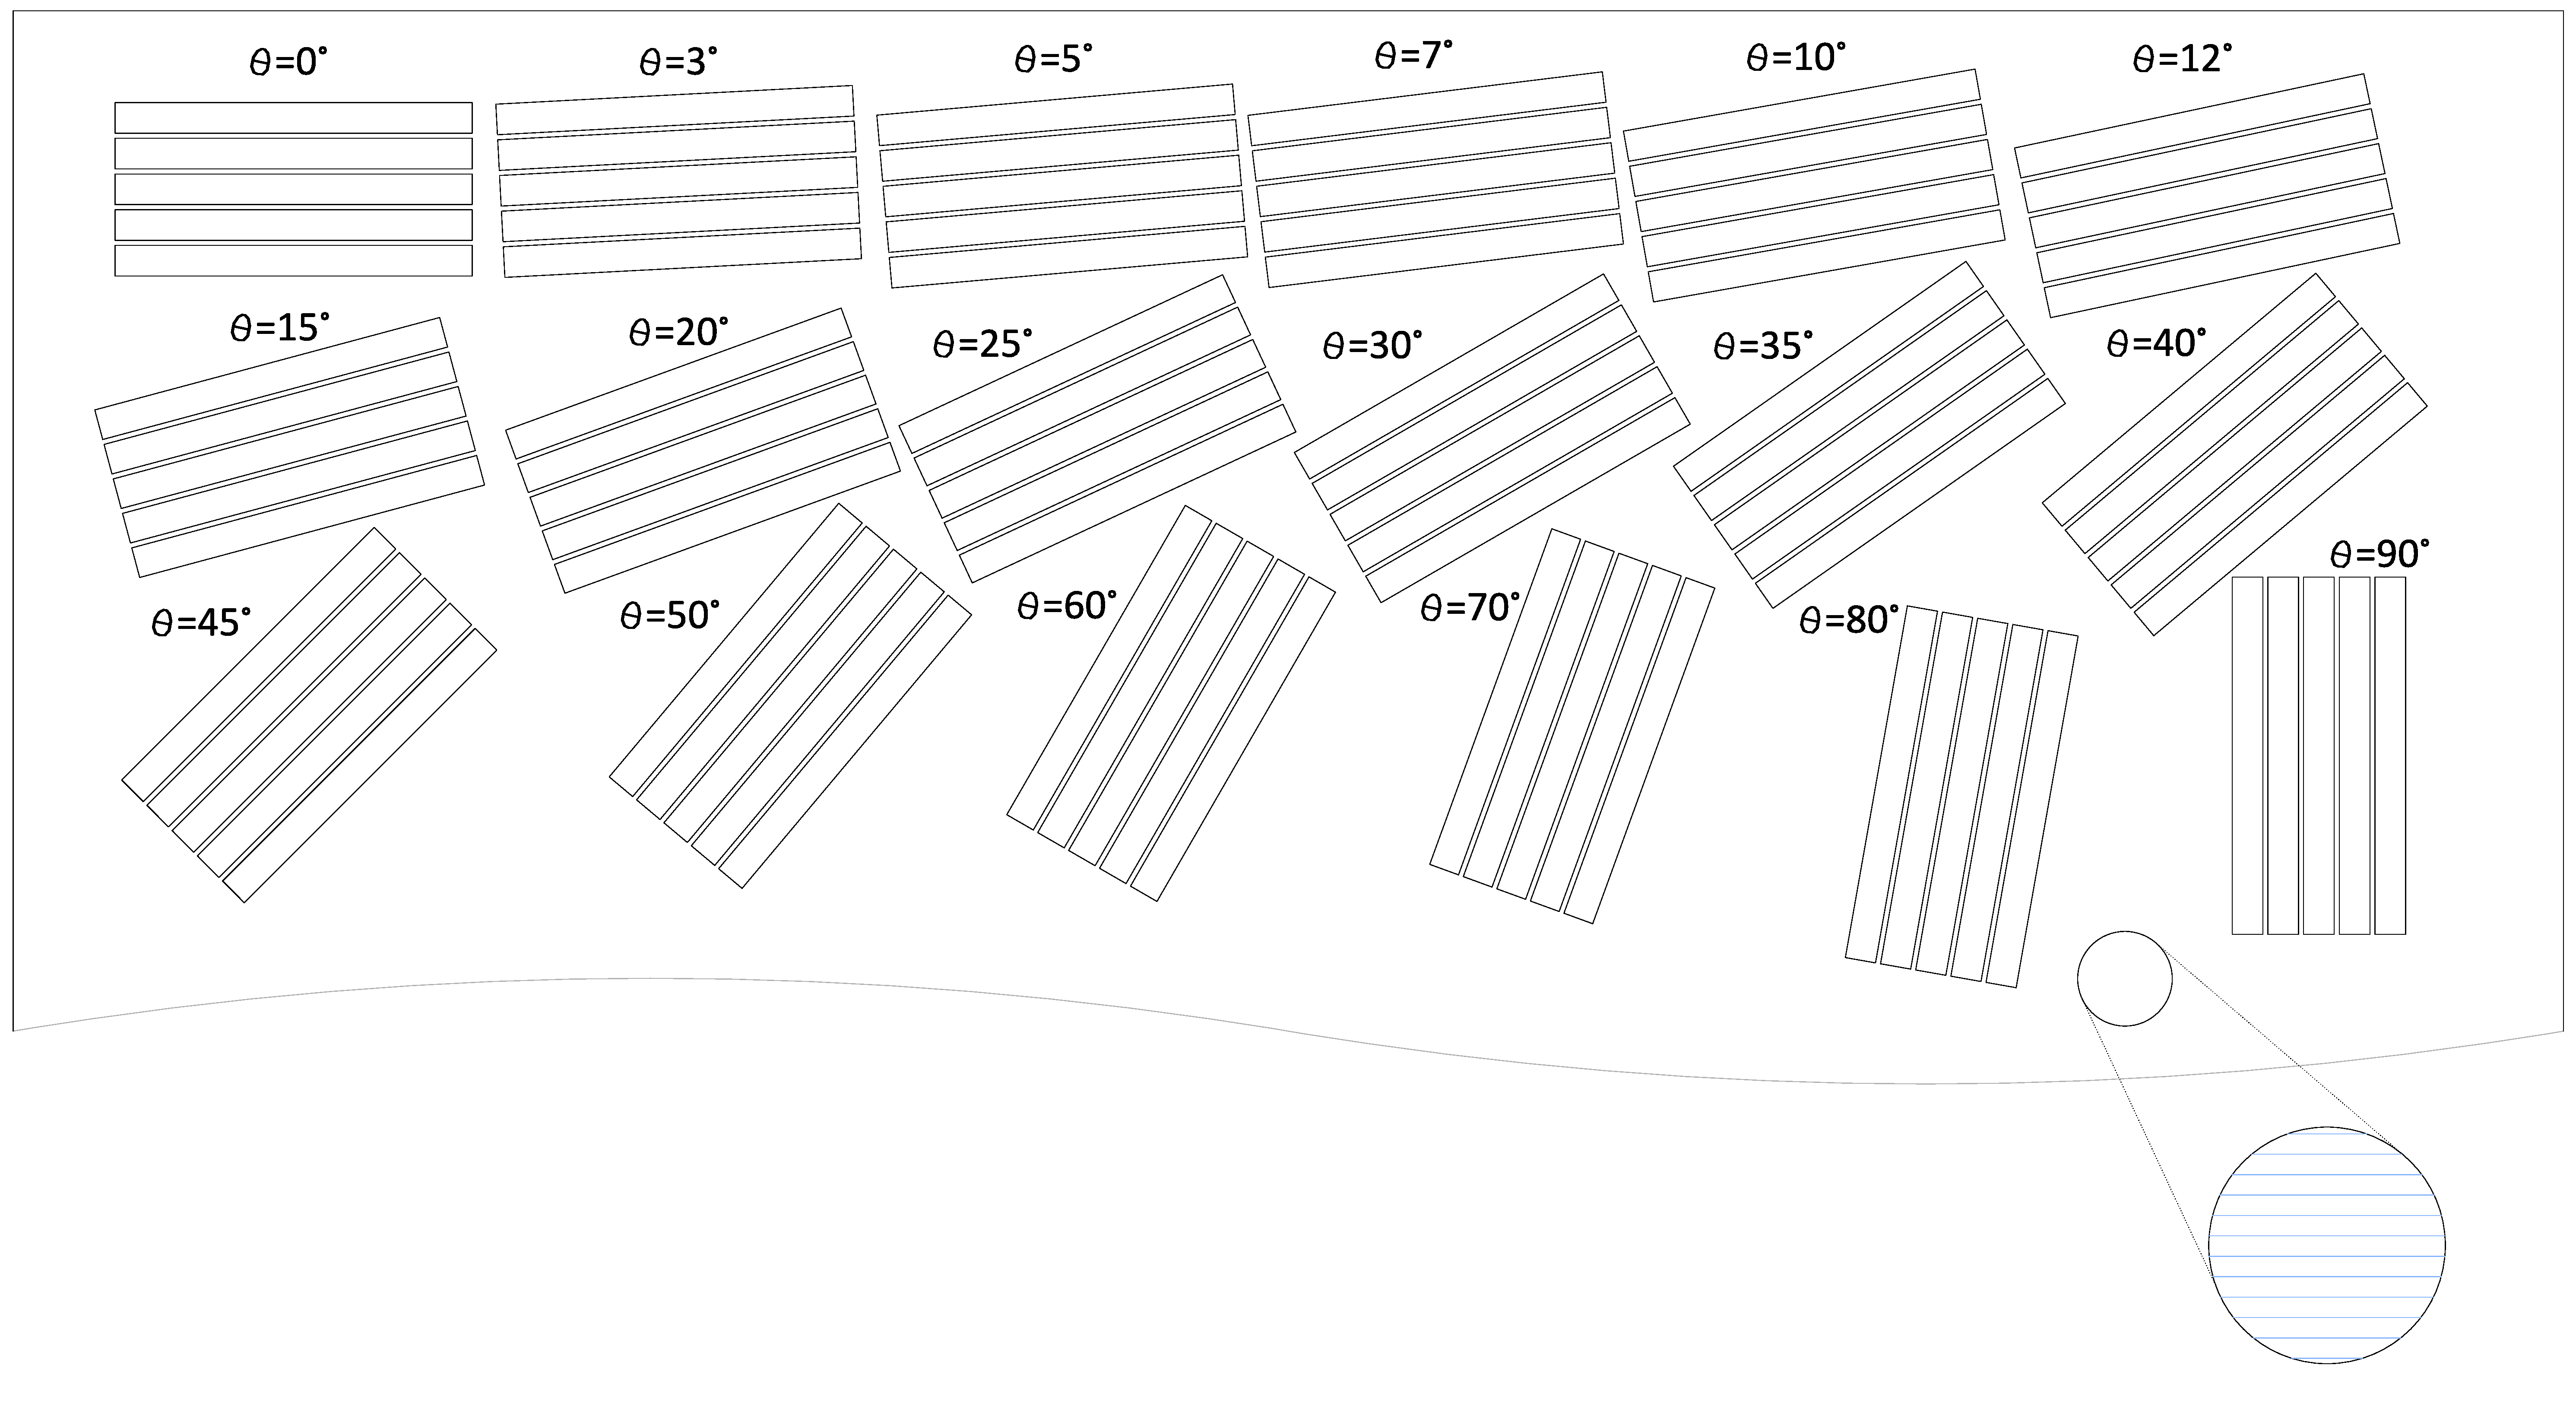
\includegraphics[scale=0.14]{\imgpath/\currfilebase/specimen_plateA}
    \caption{Water jet cutting pattern for carbon fibre plate with fibre direction indicated in blue and off-axis angle $\theta$}
    \label{fig:specimen_plateA}
\end{figure}

\subsection{Specimen Preparation}
\label{subsec:spec_prep}

The specimen preparations include all alterations of the specimen after cutting the plate and before mounting it on the test setup. Specimens of both untabbed and tabbed form were tested on the test setup requiring different preparation steps.

\begin{minipage}[t]{\dimexpr(\distTextWidth-\distColSep)/2\relax}
    Untabbed specimen preparation:
    \begin{enumerate}
        \item Removing the specimens from the cut plate 
        \item Grinding off the remaining material from the connection to the base plate
        \item Roughening contact surface for fixture and grading
        \item Grading the field of interest
    \end{enumerate}
\end{minipage}% <- must be used if no gap
\hfill% <- use if there is a gap
\noindent
\begin{minipage}[t]{\dimexpr(\distTextWidth-\distColSep)/2\relax}
    Tabbed specimen preparation:
    \begin{enumerate}
        \item Removing the specimens and tabs from the cut plates respectively
        \item Grinding off the remaining material from the connection to the base plates for both the tabs and the specimen
        \item Roughening contact surfaces specimen tab connection and for fixture and grading
        \item Use adhesive bonding to connect the tabs to the specimens
        \item Grading the field of interest
    \end{enumerate}
\end{minipage}

\subsection{Specimen Dimensions}
\label{subsec:spec_dim}

The specimen dimensions follow the test fixture standard \cite{D6641standard}. The length of a specimen defines the gap between lower and upper part of the fixture at zero load. This gap was not varied in the scope of this thesis has been chosen to be equal to the specimen width. The resulting dimensions are shown in \autoref{fig:specimen_nx_dim_labels}.

To be able to derive the total compression stress from the compressive force one needs to devide it by the cross-section. Hence the cross-section must be known. Therefore the specimens were measured in both their thickness and width at multiple locations as depicted in \autoref{fig:specimen_nx_meas}.

\begin{figure}[!ht]
    \centering
    \begin{subfigure}[t]{\dimexpr(\distTextWidth-\distColSep)/2\relax}
        \centering
        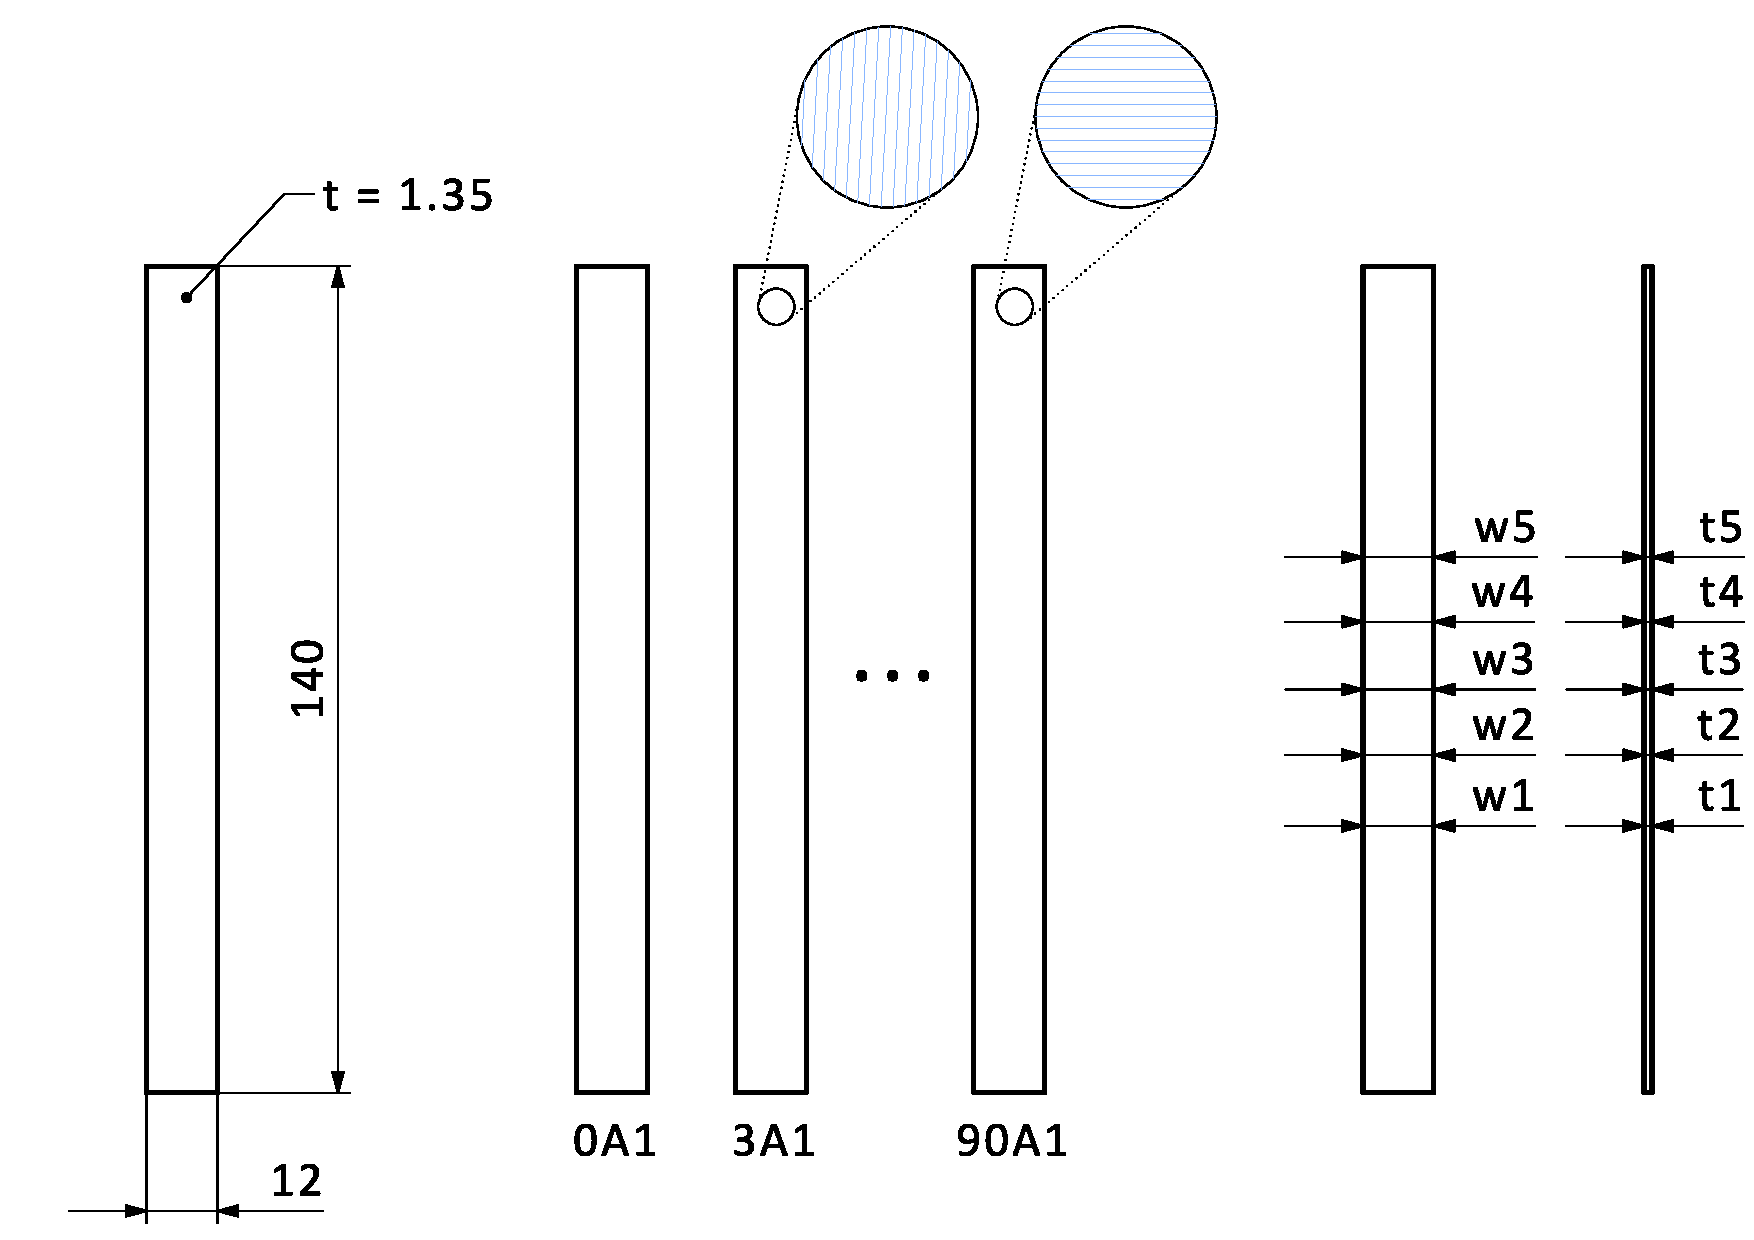
\includegraphics[%
        %trim={1cm 0.2cm 0cm 0.2cm}, % all views
        trim={1cm 0.2cm 9cm 0.2cm}, % dim and label
        %trim={1cm 0.2cm 21.5cm 3cm}, % dim
        %trim={9.5cm 1.5cm 9cm 0.2cm}, % label
        %trim={21.8cm 2.5cm 0cm 4.5cm}, % meas
        clip,scale=0.4]{\imgpath/\currfilebase/specimen}
        \caption{Specimen dimensions with example labels}
        \label{fig:specimen_nx_dim_labels}
    \end{subfigure}%
    \hfill
    \begin{subfigure}[t]{\dimexpr(\distTextWidth-\distColSep)/2\relax}
        \centering
        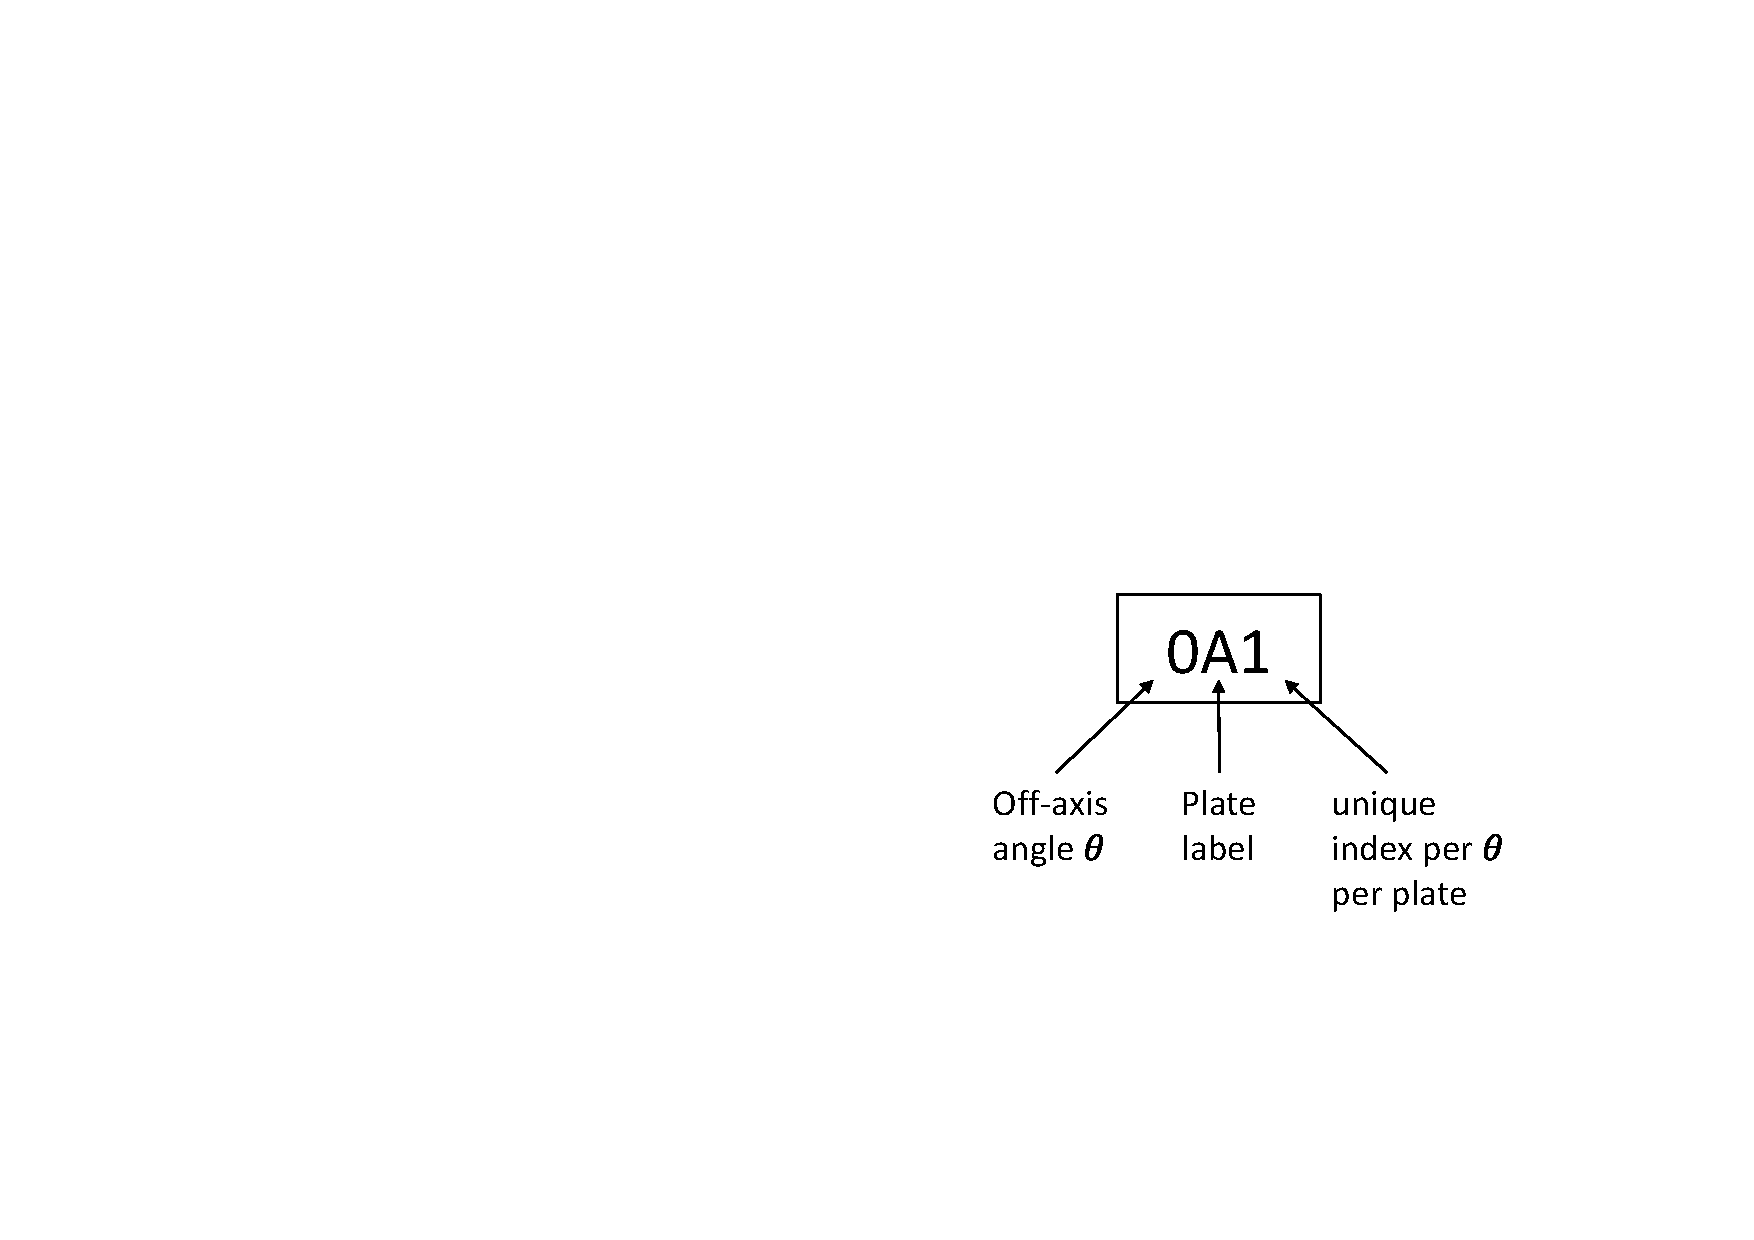
\includegraphics[scale=0.6]{\imgpath/\currfilebase/specimen_label}
        \caption{Specimen labelling system}
        \label{fig:specimen_label}
    \end{subfigure}
    \caption{Specimen dimensions and labels}
    \label{fig:specimen_dim_lab}
\end{figure}

\begin{figure}[!ht]
    \centering
    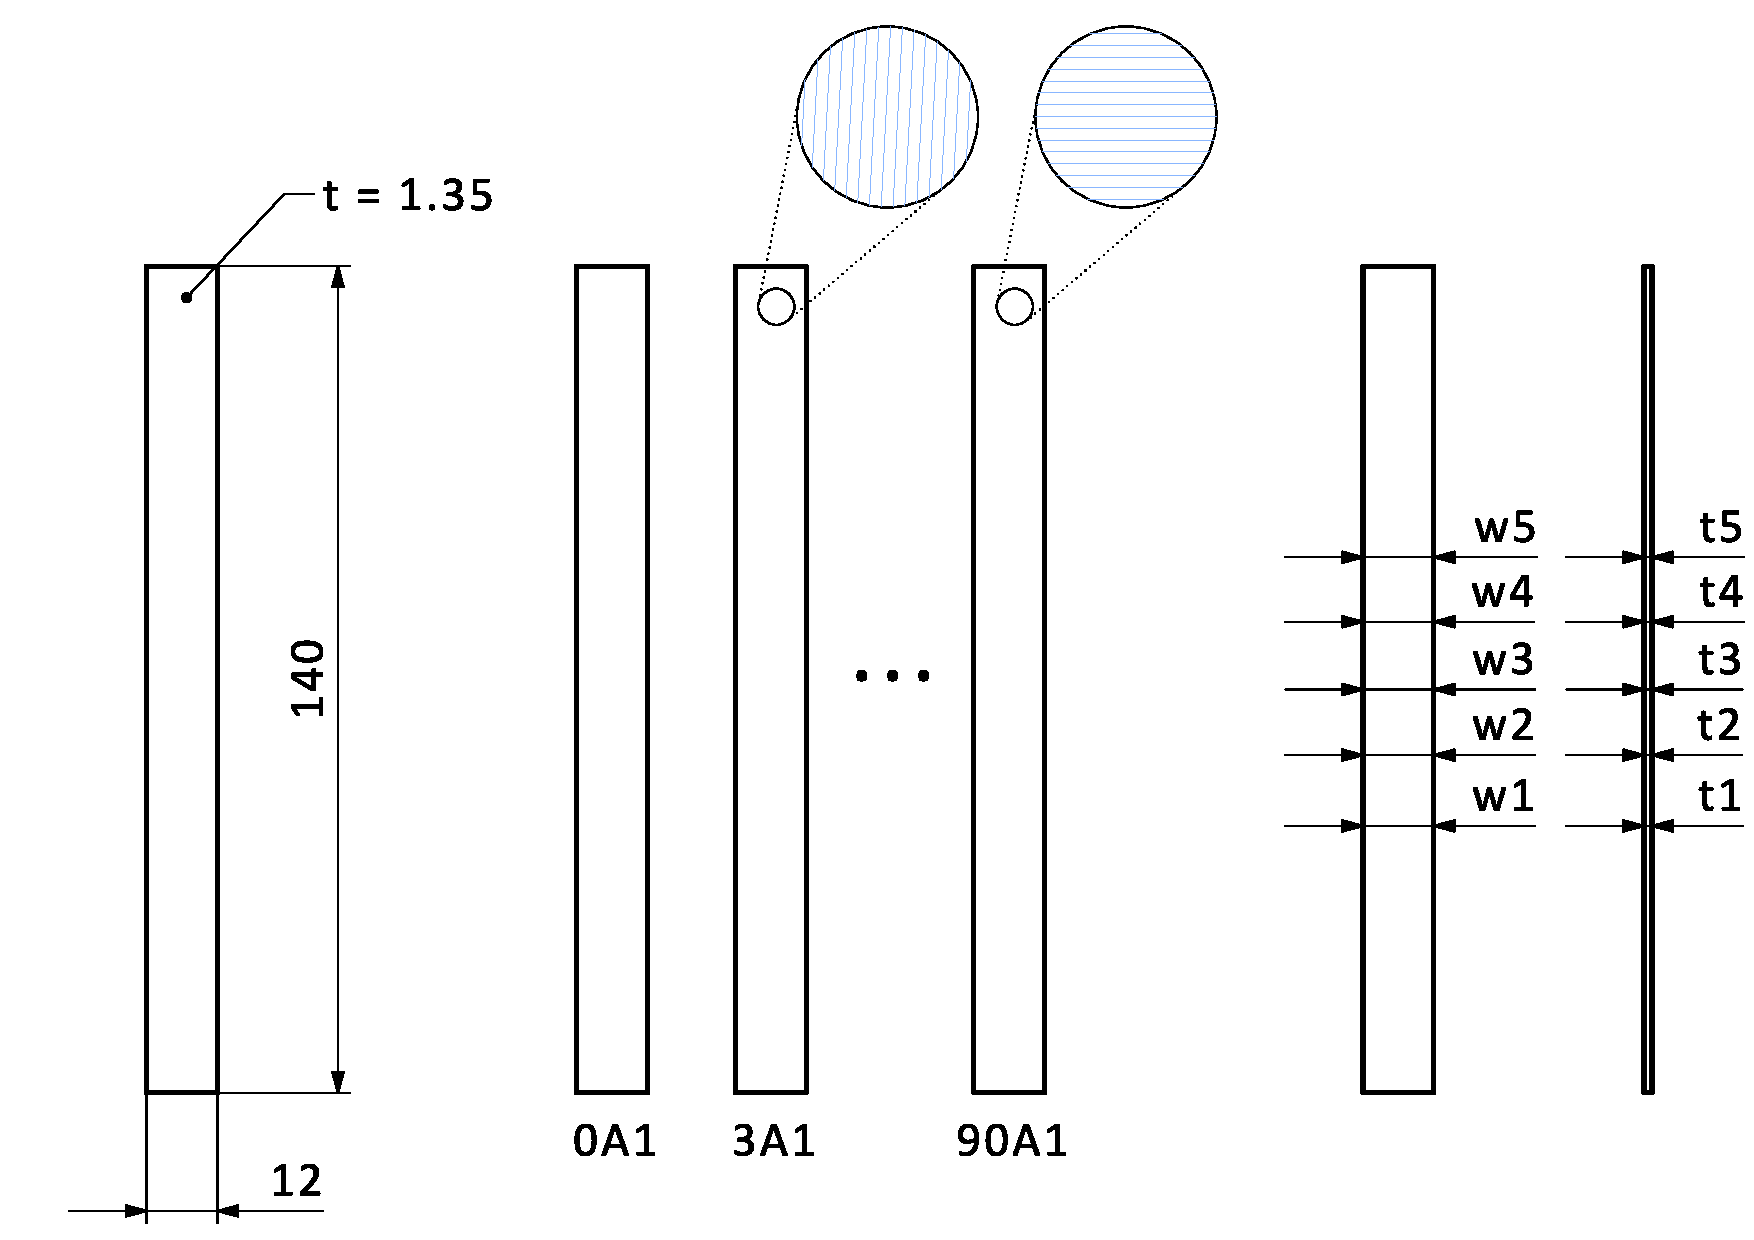
\includegraphics[%
    %trim={1cm 0.5cm 0cm 0.5cm}, % all views
    %trim={1cm 0.5cm 9cm 0.5cm}, % dim and label
    %trim={1cm 0.5cm 21.5cm 3cm}, % dim
    %trim={9.5cm 1.5cm 9cm 0.5cm}, % label
    trim={21.8cm 2.5cm 0cm 4.5cm}, % meas
    clip,scale=0.4]{\imgpath/\currfilebase/specimen}
    \caption{Specimen dimension measurements}
    \label{fig:specimen_nx_meas}
\end{figure}